% ==== BEGIN OF PREAMBLE =======================================================
% ---- document class (use appropriate driver for DIV to PS/PDF conversion):
\documentclass[12pt,a4paper]{book}

% ---- my packages
\usepackage{datetime}
\newdateformat{monthyeardate}{\monthname[\THEMONTH] \THEYEAR}

% ---- graphicx package:
\usepackage{graphicx}


% ---- natbib package:
\usepackage{natbib}
\bibpunct{(}{)}{;}{a}{}{,}  % adjust author-year citation format 


% ---- hyperref package for cross-references:
\usepackage{hyperref}
% -- USE BLACK LINKS IN PRINTOUT (uncomment the following lines if necessary):
%\hypersetup{colorlinks,%
%            linktocpage,%
%            breaklinks,%
%            citecolor=black,%
%            filecolor=black,%
%            linkcolor=black,%
%            urlcolor=black,}
% -- use color links in pdf version (comment the following lines if necessary):
\hypersetup{colorlinks,
            linktocpage,%  make page number, not text, be link on TOC, LOF & LOT
            breaklinks,%
            citecolor=blue,%
            filecolor=blue,%
            linkcolor=blue,%
            urlcolor=blue,}


% ---- caption package:
\usepackage[font=small,labelfont=bf]{caption}


% ---- subfigure package:
\usepackage[tight,nooneline,FIGTOPCAP,bf]{subfigure}
% \setlength{\subfigcaptopadj}{-6pt}  % vertical position of subfigure labels
\renewcommand{\thesubfigure}{\alph{subfigure}}
\makeatletter
    \renewcommand{\@thesubfigure}{(\thesubfigure)}  % subfigure labels:     (a)
    \renewcommand{\@@thesubfigure}{\thesubfigure}   % produced by \subref:   a
    \renewcommand{\p@subfigure}{\thefigure}         % produced by \ref:   3.1a
\makeatother


% ---- fancyhdr package:
\usepackage{fancyhdr}


% ---- some other useful packages:
% \usepackage{showkeys}  % show all keys (labels)
% \usepackage{times}     % use times new roman instead of computer modern font


% ---- page layout:
\setlength{\textheight}{24cm}
\setlength{\textwidth}{15cm}
\setlength{\topmargin}{-0.9cm}
\setlength{\headheight}{0.6cm}
\setlength{\headsep}{1cm}
\setlength{\footskip}{1cm}
\setlength{\oddsidemargin}{9.1mm}
\setlength{\evensidemargin}{-0.2mm}
\setlength{\marginparwidth}{2cm}


% ---- paragraph and line properties:
\setlength{\parindent}{0.8cm}
\setlength{\parskip}{0pt}
\linespread{1.2}
\sloppy % reduce number of word divisions and use more space between words


% ---- header format: use fancyhdr page style:
\pagestyle{fancy}
\fancyhf{}
\renewcommand{\chaptermark}[1]{\markboth{#1}{}}
\renewcommand{\sectionmark}[1]{\markright{\thesection\ #1}}
\fancyhead[LE,RO]{\thepage}
\fancyhead[LO]{\slshape \small \rightmark}
\fancyhead[RE]{\slshape \small \leftmark}
\renewcommand{\headrulewidth}{0pt}


% ---- define label format for equations, figures, and tables:
\renewcommand{\theequation}{\thechapter.\arabic{equation}}
\renewcommand{\thefigure}{\thechapter.\arabic{figure}}
\renewcommand{\thetable}{\thechapter.\arabic{table}}


% ==== END OF PREAMBLE =========================================================


% ==== BEGIN OF BODY ===========================================================
\begin{document}


% ==== START FRONT MATTER (use ROMAN numerals) =================================
\frontmatter


% ==== TITLE PAGE ==============================================================
% ---- include tex-file (CHOOSE APPROPRIATE FILE):
%!TEX root = thesis.tex
\begin{titlepage}
\begin{center}

% ---- main title
~\\[15mm]
{\Huge  {\bf Testing the importance of explicit glacier dynamics for
future glacier evolution in the Alps}}\\[5mm]


% ---- subtitle (if necessary):
% {\LARGE {\bf Subtitle}\\[15mm]


% ---- type of thesis:
{\Large \textsc{Master's Thesis}} \\[15mm]


% ---- field of study:
{\large in Atmospheric Sciences} \\[15mm]


% ---- institution:
{\large Submitted to the} \\[2mm]
{\Large \textsc{Department of Atmospheric and Cryospheric Sciences}} \\[2mm]
{\large of the} \\[2mm]
{\Large \textsc{University of Innsbruck}} \\[15mm]


% ---- degree:
{\large in Partial Fulfillment of the Requirements for the Degree of} \\[2mm]
{\Large \textsc{Master of Science}} \\[15mm]


% ---- author:
{\large by} \\[2mm]
{\Large \textsc{Moritz Oberrauch}} \\[15mm]


% ---- advisor:
{\large Advisor} \\[2mm]
{\large Fabien Maussion, PhD} \\[15mm]


% ---- location, date:
{\large Innsbruck, \monthyeardate{\today}}


\end{center}
\end{titlepage}

\newpage
~\thispagestyle{empty}
\newpage
% ---- start page numbering again:
\setcounter{page}{1}


% ==== DEDICATION ==============================================================
% ---- include tex-file:
%!TEX root = thesis.tex
% \addcontentsline{toc}{chapter}{Dedication}
\thispagestyle{plain}

\begin{flushright}
 \Large\em\null\vskip5cm To Psycho \\
 \large And all others who try to move their toes individually
\end{flushright}

\newpage
\thispagestyle{plain}


% ==== PREFACE =================================================================
% ---- include tex-file:
% %!TEX root = thesis.tex
\chapter*{Preface}
\addcontentsline{toc}{chapter}{Preface}
\thispagestyle{plain}

If I need a preface, I'll come back here later...

\begin{flushright}
\textit{Moritz Oberrauch}

\textit{Innsbruck, \monthyeardate{\today}} 
\end{flushright}

% \newpage
% \thispagestyle{plain}


% ==== ABSTRACT ================================================================
% ---- set some counters to zero:
\setcounter{equation}{0}
\setcounter{table}{0}
\setcounter{figure}{0}
% ---- include tex-file:
%!TEX root = thesis.tex
\chapter*{Abstract}
\addcontentsline{toc}{chapter}{Abstract}
\thispagestyle{plain}

% The abstract is a short summary of the thesis. It announces in
% a brief and concise way the scientific goals, methods, and most important
% results. The chapter ``conclusions'' is not equivalent to the abstract!
% Nevertheless, the abstract may contain concluding remarks. The abstract
% should not be discursive. Hence, it cannot summarize all aspects of the thesis
% in very detail. Nothing should appear in an abstract that is not also
% covered in the body of the thesis itself. Hence, the abstract should be the
% last part of the thesis to be compiled by the author.

% A good abstract has the following properties: \emph{Comprehensive:} All major
% parts of the main text must also appear in the abstract. \emph{Precise:}
% Results, interpretations, and opinions must not differ from the ones in the main
% text. Avoid even subtle shifts in emphasis. \emph{Objective:} It may contain
% evaluative components, but it must not seem judgemental, even if the thesis
% topic raises controversial issues. \emph{Concise:} It should only contain the
% most important results. It should not exceed 300--500 words or about one page.
% \emph{Intelligible:} It should only contain widely-used terms. It should
% not contain equations and citations. Try to avoid symbols and acronyms (or at
% least explain them). \emph{Informative:} The reader should be able to quickly
% evaluate, whether or not the thesis is relevant for his/her work.

% An Example: The objective was to determine whether \dots (\emph{question/goal}).
% For this purpose, \dots was \dots (\emph{methodology}). It was found that \dots
% (\emph{results}). The results demonstrate that \dots (\emph{answer}).

Global glacier models are imperative to project future glacier ice mass loss and the accompanied sea level rise. Glaciers are controlled by their mass balance and the resulting ice flow.
The scarcity of ice volume observations makes the calibration, and especially validation, of geometry models difficult. As a consequence, most global model use \vas{} relations instead of a dedicated ice physic model. Over the last years, the increasing accuracy and coverage of global data inventories, in combination with new and automated methods, as well as increased computing power allowed for the development of more sophisticated models. This study compares the global glacier model based on scaling relations by \citet{Marzeion2012b} to the globally applicable flowline model based on the Shallow Ice Approximation by \citet{Maussion2019} under controlled boundary conditions.

The reimplemented \vas{} model is able to correctly simulate glacier changes in response to various climatic forcings. The results are conceptually correct and comparable to those of the flowline model. The 21st century projection for South Asia West (RGI region 14) forced by CMIP6 data estiamtes an ice loss relative to 2020 between -27\SI{\pm3}{\percent} under SSP1-2.6 and -37\SI{\pm4}{\percent} under SSP5-8.5 for the \vas{} model, and -26\SI{\pm8}{\percent} under SSP1-2.6 and -48\SI{\pm10}{\percent} under SSP5-8.5 for the flowline model. For Central Europe the projected ice loss is much higher with up to -84\SI{\pm5}{\percent} estimated by the \vas{} model and -98\SI{\pm2}{\percent} estimated by the flowline model for SSP5-8.5, and the differences between the models are larger. The differences between \vas{} model and flowline model are eventhe introduction of ice physics modules does not devalue more pronounced for idealized equilibrium experiments and can be attributed to a missing mass-balance-elevation feedback and the overestimation of model-internal time scales. Additionally, these too long time scales result in oscillating adjustments of glacier geometries to step changes in climate. Nevertheless, the \vas{} model performane is still competitive for global applications and the introduction of ice physics modules does not complete devalue the scaling approach.


\newpage
\thispagestyle{plain}


% ==== TABLE OF CONTENTS =======================================================
~
\newpage
\addcontentsline{toc}{chapter}{Contents}
\tableofcontents
\newpage
\thispagestyle{plain}


% ==== START MAIN MATTER (use ARABIC numerals) =================================
\mainmatter


% ==== INTRODUCTION (CHAPTER 1) ================================================
% ---- set some counters to zero:
\setcounter{equation}{0}
\setcounter{table}{0}
\setcounter{figure}{0}
% ---- include tex-file:
%!TEX root = thesis.tex
\chapter{Introduction}\label{chap1}
\thispagestyle{plain}

% ====SECTION 1 ================================================================
\section{Motivation}
The chapter Introduction leads the reader into the subject matter
of the thesis. It is sometimes called
Statement/Formulation/Definition/Presentation of the Problem. It may start with
a so-called Motivation. It also contains the State of Knowledge or State
of Research which is based on a literature survey (see section \ref{1sec:2}).
Further, it contains the Scientific Questions and/or the Goals that are
addressed in the main part of the thesis (see section \ref{1sec:3}). Finally,
it provides an Outline of the science thesis (see end of section \ref{1sec:3}).


% ==== SECTION 2 ===============================================================
\section{State of Research}\label{1sec:2}

Based on the literature survey, the writer draws a picture of the existing
knowledge in a specific field and points to open questions. Hence, after this
survey the Introduction will ultimately culminate in the formulation of specific
scientific questions/goals addressed in the thesis (see section \ref{1sec:3}).

To cite a certain source (e.g., a paper) use the citation commands
\verb|\citet| and \verb|\citep| of the \verb|natbib|
package.\footnote{
\url{http://www.ctan.org/tex-archive/macros/latex/contrib/natbib/natnotes.pdf}}
Together with the bibliography style \verb|ametsoc.bst|, which is
included in the \LaTeX{} manuscript template for AMS journals\footnote{
\url{http://www.ametsoc.org/PUBS/journals/AMS_Latex_V3.0.tar.gz}}, \verb|natbib|
produces citations in the author-date format together with a list of
references that fulfill the AMS citation standard.\footnote{
\url{http://www.ametsoc.org/PUBS/journals/author_reference_guide.pdf}}

As an example, you can cite papers like \citet{hann66Aag} and \citet{scha93Aag}
which have to be specified in your BibTeX database file (in this case it is
\verb|mybibfile.bib|). More than one article of the same author can be cited
like here: \citet{hoin85Aag,hoin90Aag} studied foehn winds.

You may want to split your review of the literature into several sections.
Further, use paragraphs to structure your introduction. If you like to cite
papers in brackets (\emph{passive citations}) you can do this
as in the following sentence: Gap flows have been studied in the Strait
of Gibraltar \citep{scor52Aag,dorm95Aag}, in the French Rh\^one Valley
\citep{pett82Aag}, near Hokkaid\=o in Japan \citep{arak69Aag}, near
Unimak Island in the Aleutian Chain \citep{pan-99Aag}, and in the Howe
Sound of British Columbia \citep{jack94Aag,jack94Bag}. Citation of a
Dissertation: The gap flow in the Wipp Valley has been studied by
\citet{gohm03Aag}. Citation of a conference paper: \citet{gohm06Aag}
investigated the boundary layer structure in the Inn Valley. Citation of an
online document: The AMS provides a guideline for preparing citations and
references \citep{ams-09Aag}.


% ==== SECTION 3 ===============================================================
\section{Goals and Outline}\label{1sec:3}

After the literature survey the Introduction will ultimately culminate in the
formulation of specific scientific questions, aims or \emph{goals}. Hence, near
the end of the Introduction there will often appear sentences like:\\[1ex]
\dots The goal of the investigation thus became trying to find out if \dots\\
\dots For this reason it appeared reasonable to attempt \dots\\
\dots It therefore became necessary to clarify whether \dots\\ 

Instead of describing the goals in one paragraph, you may want to structure them
with the \verb|itemize| command:
\begin{itemize}
\item[(1)] First goal.
\item[(2)] Second goal.
\item[(3)] Third goal.
\end{itemize}

The so-called SMART
criteria\footnote{\url{http://en.wikipedia.org/wiki/SMART_criteria}} might be
used as a guideline to define reasonable goals. Here, the acronym SMART
describes the properties of ``good'' goals: \underline{s}pecific,
\underline{m}easurable, \underline{a}ttainable, \underline{r}elevant,
\underline{t}ime-bound.

The introduction may also describe briefly the methodology chosen and the
materials (e.g., data, instruments, etc.) used. However, a detailed description
will follow in the main part (see chapter \ref{chap2}).

Finally you should present an \emph{outline} of your science thesis. Explain
what the reader will find in the following chapters. For example, chapter
\ref{chap2} describes the methodology. The results are presented
in chapter \ref{chap3}. A discussion is provided in chapter \ref{disc} and the
conclusions are drawn in chapter \ref{concl}.

\newpage
\thispagestyle{plain}


% ==== CHAPTER 2 ===============================================================
% ---- set some counters to zero:
\setcounter{equation}{0}
\setcounter{table}{0}
\setcounter{figure}{0}
% ---- include tex-file:
%!TEX root = thesis.tex
\chapter{Methodology}\label{chap2}
\thispagestyle{plain}

This chapter provides a detailed description of the methodology. It is
sometimes called Experimental Section. Depending on the subject it is a
``synonym'', e.g., for Theoretical Section, Computational Methods, Model
Description and Setup, Field Work, and so on. Hence, this chapter contains a
description of \emph{what has been done} in order to address the scientific
question raised in the chapter Introduction. However, it does \emph{not} contain
the results! 


% ==== SECTION 1 ===============================================================
\section{Experimental Set-up}\label{2sec:1}
Depending on the topic of the science thesis, this chapter may contain a
description of the experimental set-up, the field experiment,
datasets, instruments, measurement procedures, analysis techniques, calibration
and quality control, and other things. In case of a modeling study it may
contain the formulation and derivation of model equations, the formulation of
initial and boundary conditions, the data used to drive and validate the model,
an overview of the model set-up (e.g., parameter set-up), modifications of the
``original'' model code, a description of relevant parameterizations,
a theoretical background needed for the interpretation of model results.


% ==== SECTION 2 ===============================================================
\section{Model Equations}\label{2sec:2}

\subsection{Subsection}
Use subsections to structure your thesis. The first and second component of the
momentum equation is shown in equation (\ref{2equ:1}) and (\ref{2equ:2}),
respectively. Together with (\ref{2equ:3}) they form the set of shallow-water
equations implemented in a numerical model.

\subsubsection{Subsubsection}
You can also use ``subsubsections''. However, they do not carry a separate
heading number and they do not appear in the Table of Contents.

\subsection{Equation}
As an example for the \verb|equation| environment, I show the equations used in
the numerical shallow-water model (SWM) developed by
\citet{scha93Aag,scha93Bag}:
% ---- equation 1:
\begin{equation}
\frac{D\hat{u}}{D\hat{t}}+\frac{\partial(\hat{h}+\hat{H})}
                               {\partial\hat{x}}=0,
\label{2equ:1}
\end{equation}
% ---- equation 2:
\begin{equation}
\frac{D\hat{v}}{D\hat{t}}+\frac{\partial(\hat{h}+\hat{H})}
                               {\partial\hat{y}}=0,
\label{2equ:2}
\end{equation}
% ---- equation 3:
\begin{equation}
\frac{\partial\hat{H}}{\partial\hat{t}}+\frac{\partial(\hat{u}\hat{H})}
                                             {\partial\hat{x}}
                                       +\frac{\partial(\hat{v}\hat{H})}
                                             {\partial\hat{y}}
                                                =0,
\label{2equ:3}
\end{equation}
with the non-dimensional variables (henceforth generally labelled with hats)
$\hat{u}$ and $\hat{v}$ as the two horizontal velocity components, $\hat{H}$ and
$\hat{h}$ as fluid layer depth and terrain height, respectively,
$\hat{Z}=\hat{h}+\hat{H}$ as fluid layer height, and $\hat{t}$ as time.
Equations~(\ref{2equ:1})--(\ref{2equ:3}) are non-dimensionalized with the
following scales: a typical length $L$ for the horizontal length scale, the
initial far-upstream depth of the fluid layer $H_{\infty}$ (with $h_{\infty}=0$)
for the vertical length scale, the phase speed of linear gravity waves
$\sqrt{g^*H_{\infty}}$ for the velocity scale, and the time scale
$L/\sqrt{g^*H_{\infty}}$.

\newpage
\thispagestyle{plain}


% ==== CHAPTER 3 ===============================================================
% ---- set some counters to zero:
\setcounter{equation}{0}
\setcounter{table}{0}
\setcounter{figure}{0}
% ---- include tex-file:
%!TEX root = thesis.tex
\chapter{Results}\label{chap3}
\thispagestyle{plain}

This chapter contains a detailed description of your findings. It shows
\emph{what has been found} to answer the scientific questions. Hence, it
consists of the author's original contributions. This chapter is the
``heart'' of a science thesis.


% ==== SECTION 1 ===============================================================
\section{Some Important Things to Know}\label{3sec:1}

It is important to differentiate between \emph{facts} and \emph{interpretations}
and between \emph{your contributions} and \emph{those of others}! Facts and
your contributions are part of this chapter. Interpretations and contributions
of others should be rather part of the chapter Discussion.


\subsection{Experimental Parts in the Chapter Results}
Experimental details should only appear in the chapter Results to the
extent necessary to ensure comprehension. Painstaking descriptions of
instruments, analysis procedures, field conditions, etc., should be part of the
chapter Methodology. However, absolutely necessary is information that shows
the \emph{reliability} of the findings and the \emph{robustness} of an
innovation (e.g., a new analysis technique).


\subsection{Numerical Results or so-called Data}
Results are more than simply numbers! They are tiny but unique
\emph{messages}. Data should not only be made ``visible'' (e.g., in
figures, such as in Fig.~\ref{fig:1}) but should also be made
\emph{articulate}.


\subsection{Order of Presentation}
Use chapters and (sub)sections to separate, e.g., various topics,
questions, and problems, or to separate measurements from calculations. 
Arrange information in a consistent way, e.g., from simple to complex, from
small to large (or vice versa in terms of scales: e.g., from
synoptic-scale to micro-scale), from \emph{most important} (central) to
\emph{least important} (peripheral). Arrange the material in order to maximize
impact rather than sticking to a strict chronological order. Try to tell a story
that consists of a beginning, followed by a gradual unfolding, and a
``happy end''.


\subsection{Cross-References}
You can always refer to other parts of your thesis like in the following
example: See chapter \ref{chap2} or section \ref{1sec:3} or
Fig.~\ref{fig:1} or Table~\ref{tab:1} or equation~(\ref{2equ:1}).


\section{Figure}\label{3sec:2}
Figure \ref{fig:1} shows an example for an EPS figure with two panels. The
topography of the Wipp Valley and Inn Valley is shown in Fig.~\ref{fig:1a}.
Figure~\ref{fig:1b} shows the time series of potential temperature at two
stations. In order to refer to a certain range of figure panels write, e.g.,
Fig.~\ref{fig:1a}--\subref{fig:1b}.


\begin{figure}[!tp]
\centering
\figuretopcapfalse
\subfigure[][]{
  \label{fig:1a}  
  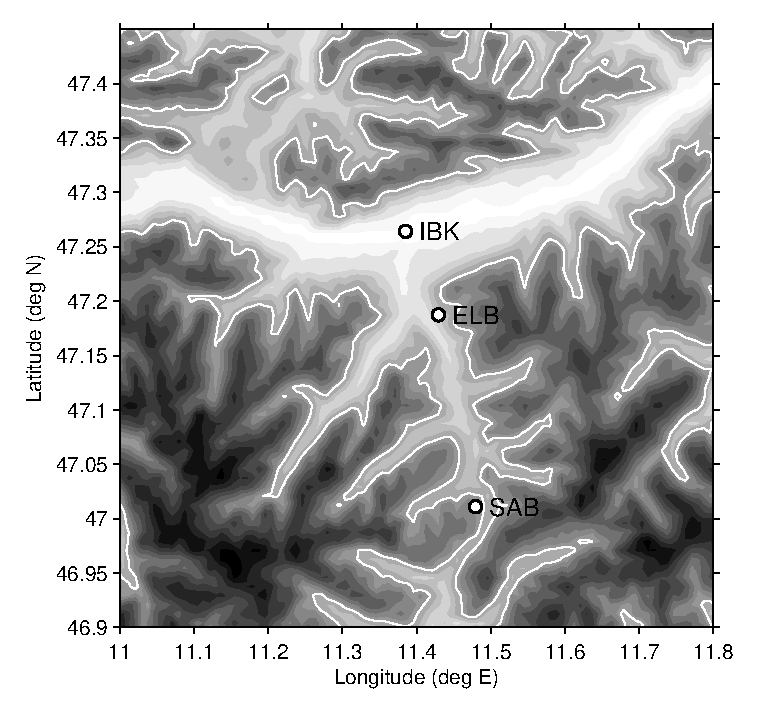
\includegraphics[width=0.48\textwidth]{figure_topo.eps}
}
\subfigure[][]{
  \label{fig:1b}
  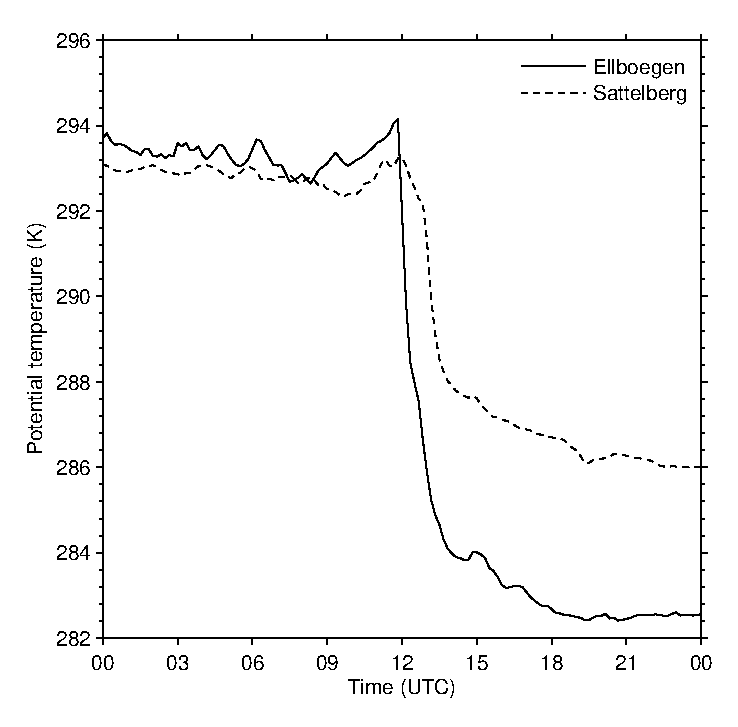
\includegraphics[width=0.47\textwidth]{figure_theta.eps}
}
\caption{(\subref{fig:1a}) Topographic map of the target area: Gray shaded
elevations contours with increments of 200~m starting at 400~m~MSL and a white
elevation contour line at 1600~m MSL. (\subref{fig:1b}) Time series of potential
temperature (K) at Ellboegen (solid line) and Sattelberg (dashed line) from 00
UTC 06 November to 00 UTC 07 November 1999. Labels in (\subref{fig:1a}) mark the
location of Innsbruck (IBK), Ellboegen (ELB), and Sattelberg
(SAB).}\label{fig:1}
\end{figure}


This template uses the \texttt{subfigure} environment with the option
\texttt{FIGTOPCAP} to place the subfigure labels (\subref{fig:1a}) and
(\subref{fig:1b}) at the top of the figure. However, since we want to have the
caption at the bottom of figure, use \verb|\figuretopcapfalse|
before the first \verb|\subfigure| command within the \texttt{figure}
environment, otherwise the figure number produced by \verb|\ref| is wrong.


\section{Table}
Table \ref{tab:1} is an example for a table that consists of several
rows and columns. Here, the \texttt{tabular} environment is used inside the
\texttt{table} environment.


\begin{table}[!htb]
\centering
\begin{footnotesize}
\renewcommand{\tabcolsep}{4pt}
\begin{tabular}{l p{3.5cm} l l l}
\hline
\hline
Parameter & Code & Description & Units & Code\\
\hline
$g$ & \verb|$g$| & acceleration due to gravity&
  m~s$^{-2}$ & \verb|m~s$^{-2}$| \\
$T_d$ & \verb|$T_d$| & dew point temperature & $^{\circ}$C & 
  \verb|$^{\circ}$C| \\
$\mathbf{v} \cdot \nabla T$ & \verb|$\mathbf{v} \cdot| \verb| \nabla T$| &
  temperature advection & K~s$^{-1}$ & \verb|K~s$^{-1}$| \\
$\vec{v} \cdot \nabla T$ & \verb|$\vec{v} \cdot| \verb| \nabla T$| & 
  temperature advection & K~s$^{-1}$ & \verb|K~s$^{-1}$| \\
$\frac{\partial p}{\partial t}$ & \verb|$\frac{\partial p}|
  \verb| {\partial t}$| & local pressure tendency & Pa~s$^{-1}$ &
  \verb|Pa~s$^{-1}$| \\
$p_0 \cos (kx - \omega t)$ & \verb|$p_0 \cos (kx| \verb| - \omega t)$| &
 wave expression & Pa & Pa \\
\hline
\end{tabular}
\end{footnotesize}
\caption{Some meteorological and mathematical parameters and expressions.}
\label{tab:1}
\end{table}


\section{Figure and Table Captions}

Figure and table captions \emph{must} contain all necessary information to
understand the \emph{content} of the figure and table, without the need of
additional text. Only in case of very complicated figures or tables, the caption
may end with a remark such as ``See text for further explanation''. The
\emph{interpretation} of the table or figure is not part of the caption, but
should be given in the main text. In order to avoid repetitions, the phrase
``As in Fig. xx, but for \dots'' is often used. Necessary information provided
in the caption is a description of
\begin{itemize}
\item shown parameters together with units,
\item date and time,
\item contour intervals,
\item location,
\item line styles and markers,
\item and others.
\end{itemize}
A list of figures and a list of tables at the beginning of the thesis (before
chapter 1) is optional.



\section{Title}

The title of your science thesis should be kept as short as possible. It should
represent an extremely compact summary of the thesis. The title should provide a
clear and complete description of the topic and should contain many keywords
(``what?'', ``how?'' and possibly ``why?''). The main title should not contain
more than 10 words. An optional subtitle may be used if necessary (all together
not more than 25 words). Important words and terms should be placed at the
beginning of the title. Avoid unspecific expressions such as
\begin{itemize}
\item[] Investigation of ...
\item[] Experiments on ...
\item[] Results of ...
\item[] Attempts to ...
\end{itemize}
Rather use expressions such as
\begin{itemize}
\item[] Influence of ... on ...
\item[] Generation of ... with ...
\item[] Dependence of ... upon ...
\item[] Optimization of ... upon ...
\end{itemize}
Avoid technical abbreviations or acronyms and special symbols such as IR
for infrared or $\theta$ for potential temperature.


\section{Abbreviations and Symbols}
Abbreviations (e.g., ECMWF) and symbols (e.g., $\vec{v}_g$) have to be
defined, i.e. explained, at the place where the \emph{first} appear in the text.
For example: The model was initialized with the operational analysis of the
European Centre for Medium-Range Weather Forecasts (ECMWF). From the ECMWF
fields of geopotential height we derive the geostrophic wind vector
$\vec{v}_g$. The change of $\vec{v}_g$ with pressure $p$ reveals the thermal
wind equation.

A list of abbreviations and a list of symbols at the beginning of the thesis
(before chapter 1) is optional.


\section{Parameters and Units}

Use italic letters for scalar quantities (e.g., $R$ and $g$), bold upright
letters or arrows for vector quantities (e.g., $\mathbf{v}_g$ or $\vec{v}_g$)
and sans-serif letters for tensors (e.g., $\mathsf{T}$). All this parameters
should be written in mathematical mode (\verb|$ ... $|). Units should be
written with normal upright letters (e.g., m~s$^{-1}$). Use spacing between
numbers and individual units (e.g., $\phi=100$~W~m$^{-2}$). Less or no spacing
is used between numbers and units in case of percent and degrees (e.g.,
10\% and 5$^{\circ}$C). See also Table~\ref{tab:1} for further examples.


\section{Footnotes}
Do not use footnotes in an extensive way. Footnotes distract the reader from the
main body of the document. Do not use footnotes for referring to literature,
rather use the author-year citation system together with a bibliography (list
of references) at the end of the thesis.

\newpage
\thispagestyle{plain}


% ==== DISCUSSION ==============================================================
% ---- set some counters to zero:
\setcounter{equation}{0}
\setcounter{table}{0}
\setcounter{figure}{0}
% ---- include tex-file:
%!TEX root = thesis.tex
\chapter{Discussion}\label{disc}
\thispagestyle{plain}

The discussion is the interpretation and evaluation of the results. It is a
comparison of your results with previous findings. It provides the answer to the
scientific questions raised in the introduction. It is the ``nerve center'' of a
thesis, whereas the chapter Results may be seen as the ``heart''.

Clearly separate between your own contributions and those of others. Provide
rigorous citations of appropriate sources! Explicitly refer to specific results
presented earlier. A certain amount of repetition is necessary. For
example, the results presented in \ref{3sec:2} suggest that \dots. Order
discussion items not chronologically but rather logically.

The chapter Results answers the question: \emph{What} has been
found? (Facts). The chapter Discussion answers the question: \emph{How} has the
result to be interpreted? (Opinion).

The most important message should appear in the first paragraph. The answer to
the key question may appear in the first sentence: e.g., did your original idea
work, or didn't it? The following questions may be answered in the discussion
section:
\begin{itemize}
\item Why is the presented method simpler, better, more reliable than previous
ones?
\item What are its strengths and its limitations?
\item How significant are the results?
\item How trustworthy are the observations?
\item Under which precondition/assumption and for which region are the
results/method valid?
\item Can the results be easily transferred to other regions or fields?
\end{itemize}

\newpage
\thispagestyle{plain}


% ==== CONCLUSIONS =============================================================
% ---- set some counters to zero:
\setcounter{equation}{0}
\setcounter{table}{0}
\setcounter{figure}{0}
% ---- include tex-file:
%!TEX root = thesis.tex
\chapter{Conclusions}\label{concl}
\thispagestyle{plain}

This chapter contains consequences that derive from your results. It may also
contain speculations. It may provide suggestions for future studies. Hence, the
conclusions may provide an outlook and list open questions. Sometimes
this chapter is part of the discussion. In such a case, the chapter reads
``Discussion and Conclusions''.

\newpage
\thispagestyle{plain}


% ==== APPENDIX ================================================================
% ---- start appendix:
\appendix
% ---- set some counters to zero:
\setcounter{equation}{0}
\setcounter{table}{0}
\setcounter{figure}{0}
% ---- include tex-file:
%!TEX root = thesis.tex

% Singel glacier test cases
\chapter{Single glacier test cases}\label{appendix_A}
\thispagestyle{plain}

The first experiment was performed as a single glacier test case on the example of Hintereisferner (RGI60-11.00897), see Section~\ref{sub:experimental_setup_test_case} for details on the experimental setup. The test case was intended to get a first qualitative impression, drawing conclusions from a single data point is, however, still questionable. Therefore, the exact same experiment was performed on five more single glaciers (Pasterze, Mer de Glace, Glacier d'Argentière, Großer Aletschgletscher, Rhonegletscher) and the results are shown here below. While there are differences between the different glaciers, all general findings presented in Section~\ref{sub:results_test_case} hold true.

\begin{figure}[p]
  \centering

  % VAS volume
  \begin{subfigure}[b]{0.476\textwidth}
    \caption{\Vas{} model, relative ice volume}
    \label{fig:Pasterze:volume_vas}
    \centering
    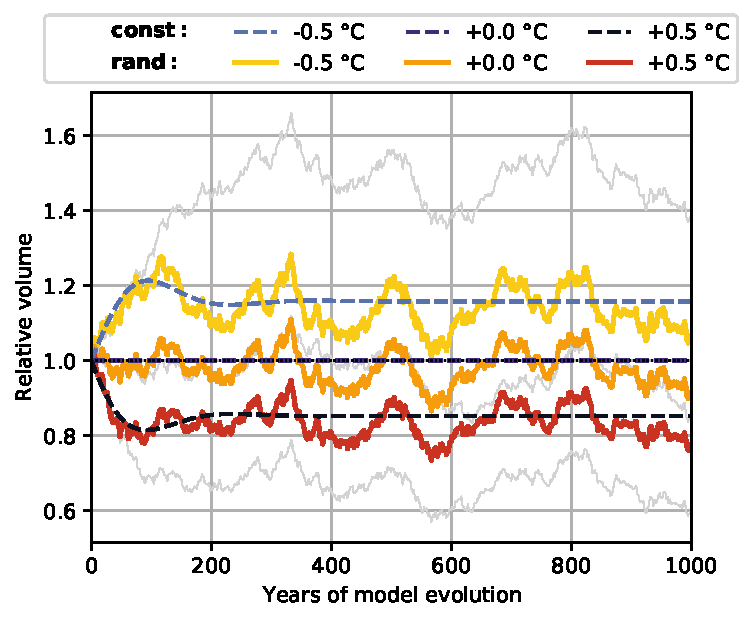
\includegraphics[width=\textwidth]{../plots/final_plots/time_series/single_glaciers/volume_norm_vas_Pasterze.pdf}
  \end{subfigure}
  \hfill
  % Flowline volume
  \begin{subfigure}[b]{0.476\textwidth}
    \caption{Flowline model, relative ice volume}
    \label{fig:Pasterze:volume_fl}
    \centering
    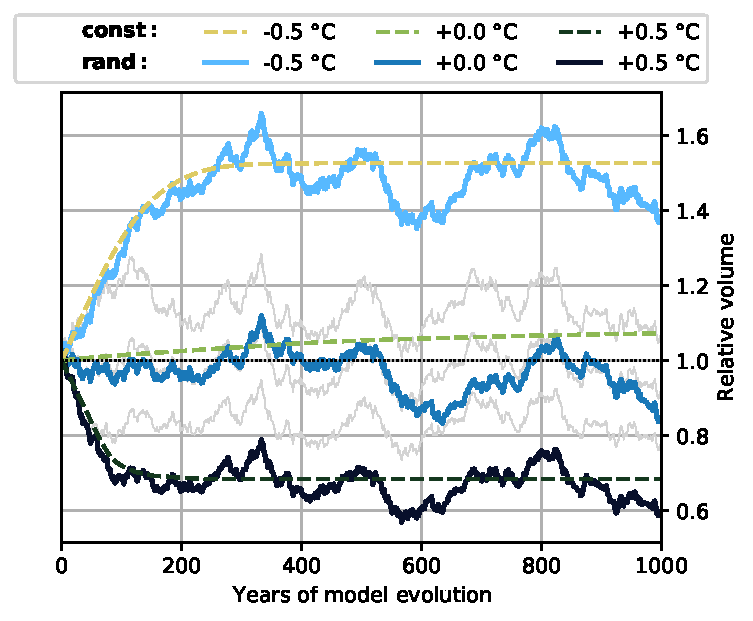
\includegraphics[width=\textwidth]{../plots/final_plots/time_series/single_glaciers/volume_norm_fl_Pasterze.pdf}
  \end{subfigure}

  % VAS area
  \begin{subfigure}[b]{0.476\textwidth}
    \caption{\Vas{} model, relative surface area}
    \label{fig:Pasterze:area_vas}
    \centering
    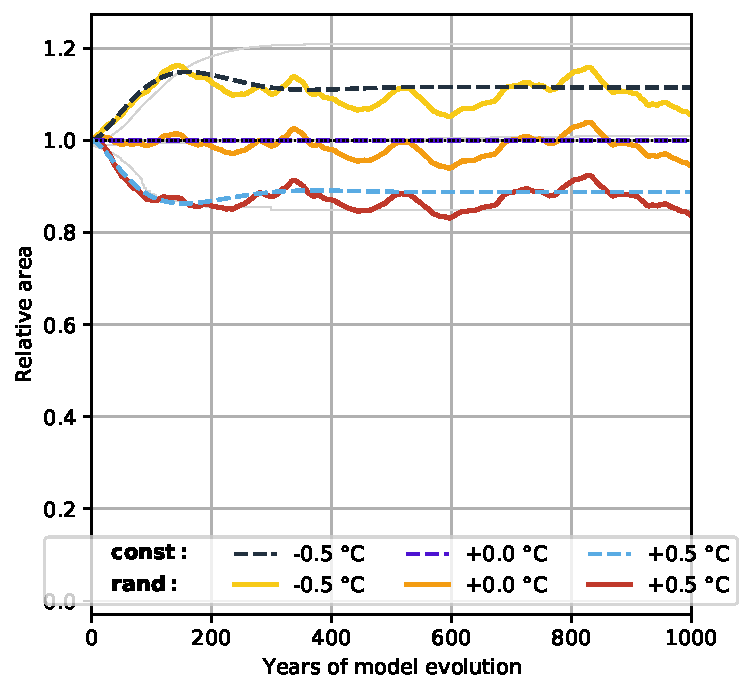
\includegraphics[width=\textwidth]{../plots/final_plots/time_series/single_glaciers/area_norm_vas_Pasterze.pdf}
  \end{subfigure}
  \hfill
  % Flowline area
  \begin{subfigure}[b]{0.476\textwidth}
    \caption{Flowline model, relative surface area}
    \label{fig:Pasterze:area_fl}
    \centering
    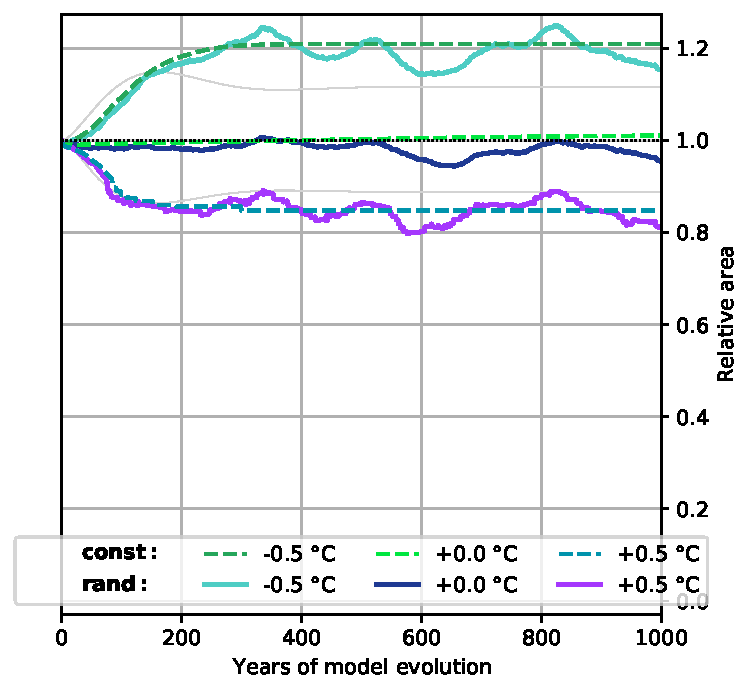
\includegraphics[width=\textwidth]{../plots/final_plots/time_series/single_glaciers/area_norm_fl_Pasterze.pdf}
  \end{subfigure}

  % VAS length
  \begin{subfigure}[b]{0.476\textwidth}
    \caption{\Vas{} model, relative glacier length}
    \label{fig:Pasterze:length_vas}
    \centering
    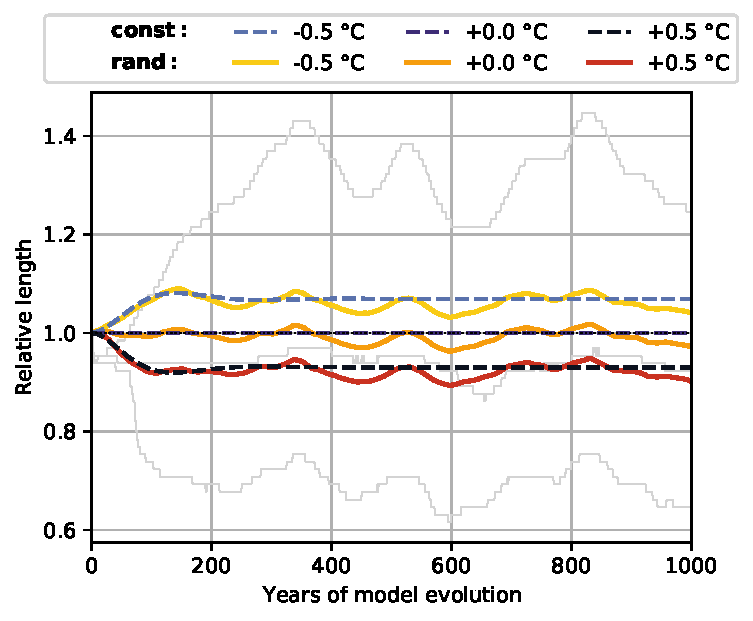
\includegraphics[width=\textwidth]{../plots/final_plots/time_series/single_glaciers/length_norm_vas_Pasterze.pdf}
  \end{subfigure}
  \hfill
  % Flowline length
  \begin{subfigure}[b]{0.476\textwidth}
    \caption{Flowline model, relative glacier length}
    \label{fig:Pasterze:length_fl}
    \centering
    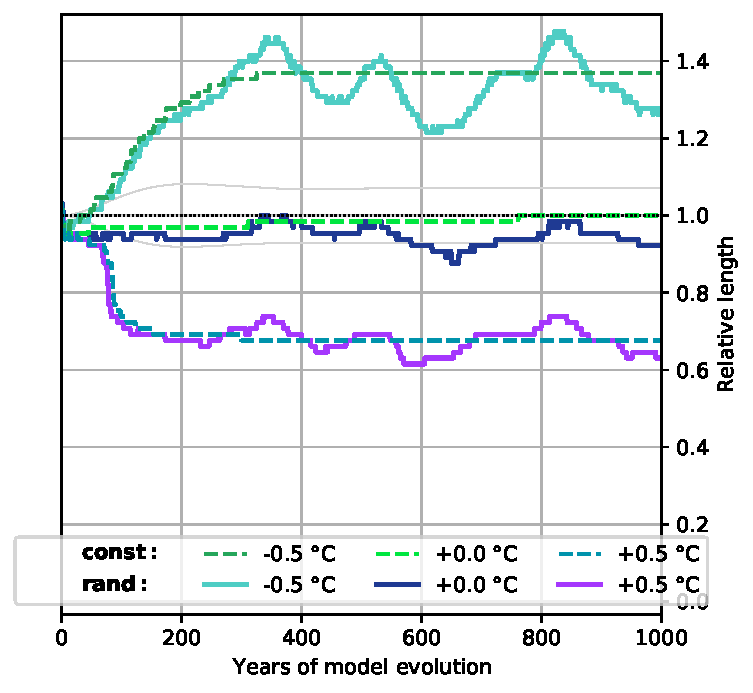
\includegraphics[width=\textwidth]{../plots/final_plots/time_series/single_glaciers/length_norm_fl_Pasterze.pdf}
  \end{subfigure}
  
  \caption{Temporal evolution of ice volume in (\subref{fig:Pasterze:volume_vas}) and (\subref{fig:Pasterze:volume_fl}), surface area in (\subref{fig:Pasterze:area_vas}) and (\subref{fig:Pasterze:area_fl}) and glacier length in (\subref{fig:Pasterze:length_vas}) and (\subref{fig:Pasterze:length_fl}) for \textbf{Pasterze (RGI60-11.00106)}. The shown values area normalized with their respective initial values. The left panels show the result of the \vas{} model, the right panels show the results of the flowline model. Solid lines represent the random climate scenarios, while dashed lines represent the constant climate scenarios. All climate scenarios are based on an equilibrium climate. The applied temperature biases of \SI{-.5}{\celsius}, \SI{0}{\celsius} and \SI{+.5}{\celsius} are color coded, see legend for details. The dotted line indicates the initial volume. The light gray lines represent the volume evolutions of the other model, to facilitate comparisons.}
  \label{fig:Pasterze}
\end{figure}

\begin{figure}[p]
  \centering

  % VAS volume
  \begin{subfigure}[b]{0.476\textwidth}
    \caption{\Vas{} model, relative ice volume}
    \label{fig:Mer_de_Glace:volume_vas}
    \centering
    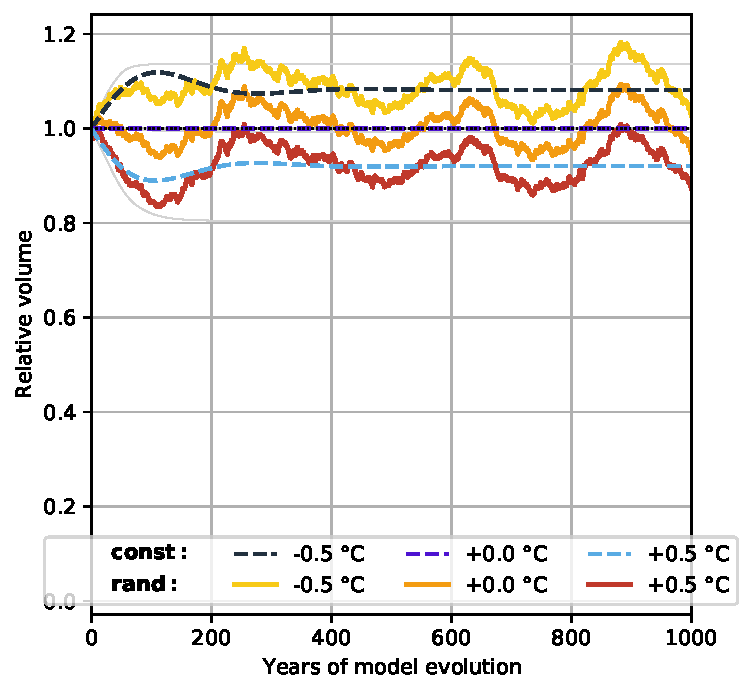
\includegraphics[width=\textwidth]{../plots/final_plots/time_series/single_glaciers/volume_norm_vas_Mer_de_Glace.pdf}
  \end{subfigure}
  \hfill
  % Flowline volume
  \begin{subfigure}[b]{0.476\textwidth}
    \caption{Flowline model, relative ice volume}
    \label{fig:Mer_de_Glace:volume_fl}
    \centering
    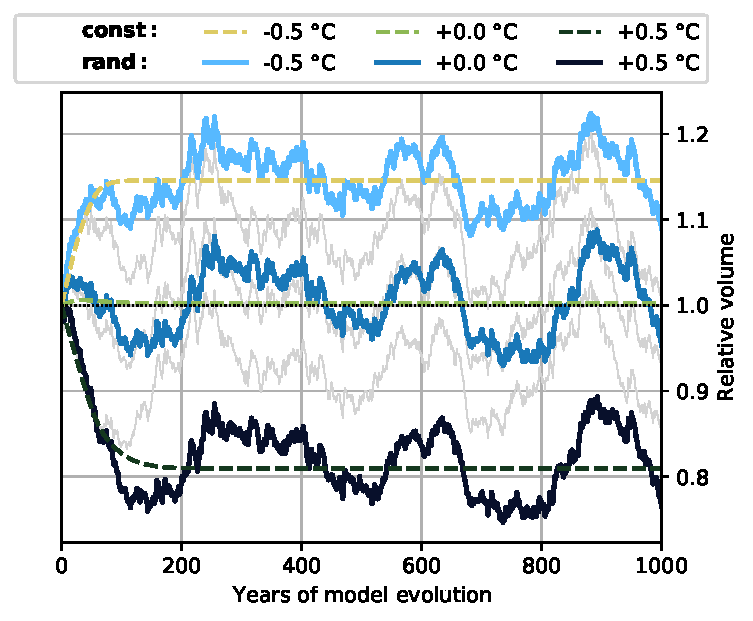
\includegraphics[width=\textwidth]{../plots/final_plots/time_series/single_glaciers/volume_norm_fl_Mer_de_Glace.pdf}
  \end{subfigure}

  % VAS area
  \begin{subfigure}[b]{0.476\textwidth}
    \caption{\Vas{} model, relative surface area}
    \label{fig:Mer_de_Glace:area_vas}
    \centering
    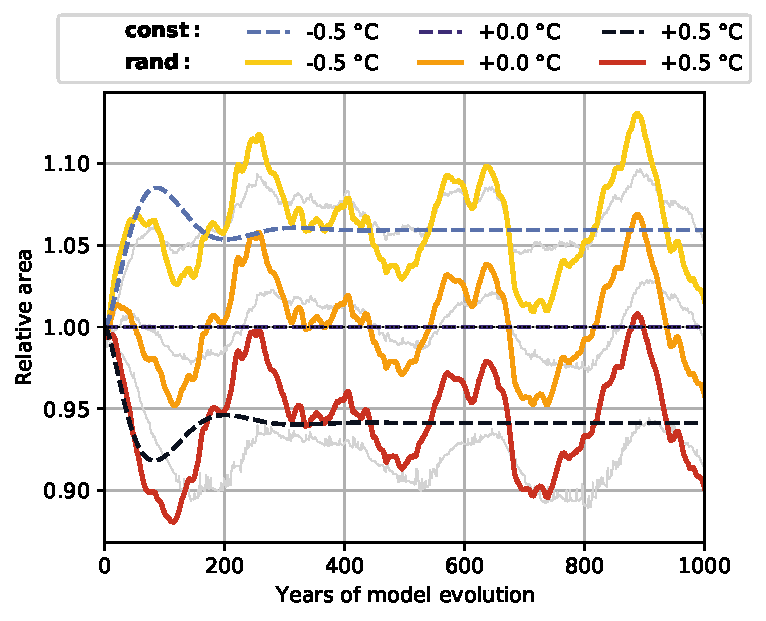
\includegraphics[width=\textwidth]{../plots/final_plots/time_series/single_glaciers/area_norm_vas_Mer_de_Glace.pdf}
  \end{subfigure}
  \hfill
  % Flowline area
  \begin{subfigure}[b]{0.476\textwidth}
    \caption{Flowline model, relative surface area}
    \label{fig:Mer_de_Glace:area_fl}
    \centering
    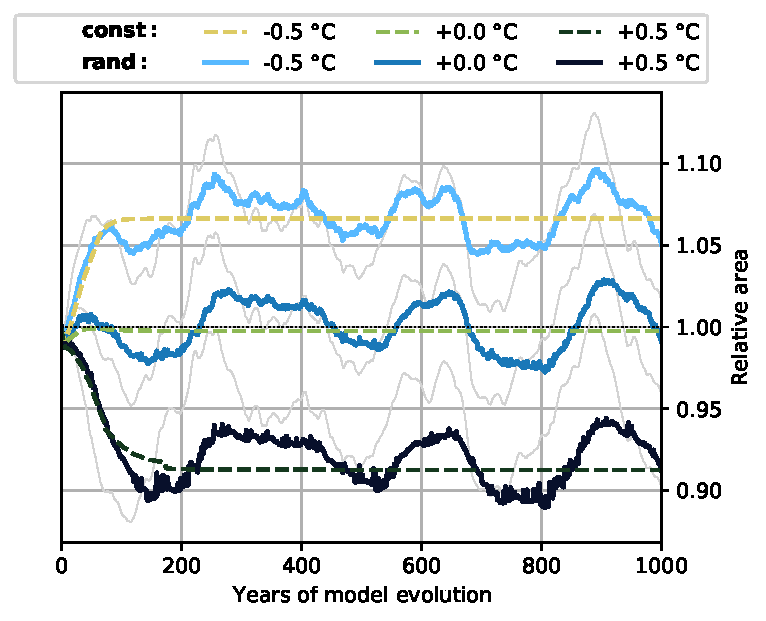
\includegraphics[width=\textwidth]{../plots/final_plots/time_series/single_glaciers/area_norm_fl_Mer_de_Glace.pdf}
  \end{subfigure}

  % VAS length
  \begin{subfigure}[b]{0.476\textwidth}
    \caption{\Vas{} model, relative glacier length}
    \label{fig:Mer_de_Glace:length_vas}
    \centering
    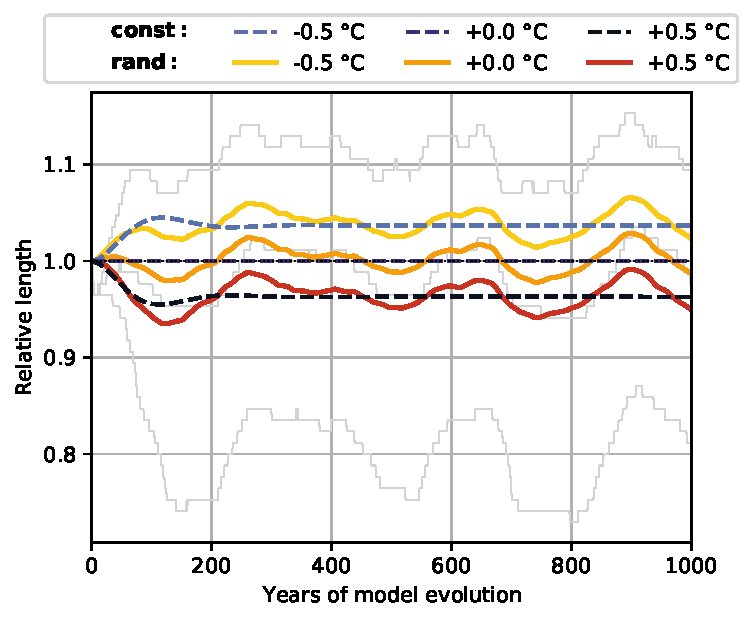
\includegraphics[width=\textwidth]{../plots/final_plots/time_series/single_glaciers/length_norm_vas_Mer_de_Glace.pdf}
  \end{subfigure}
  \hfill
  % Flowline length
  \begin{subfigure}[b]{0.476\textwidth}
    \caption{Flowline model, relative glacier length}
    \label{fig:Mer_de_Glace:length_fl}
    \centering
    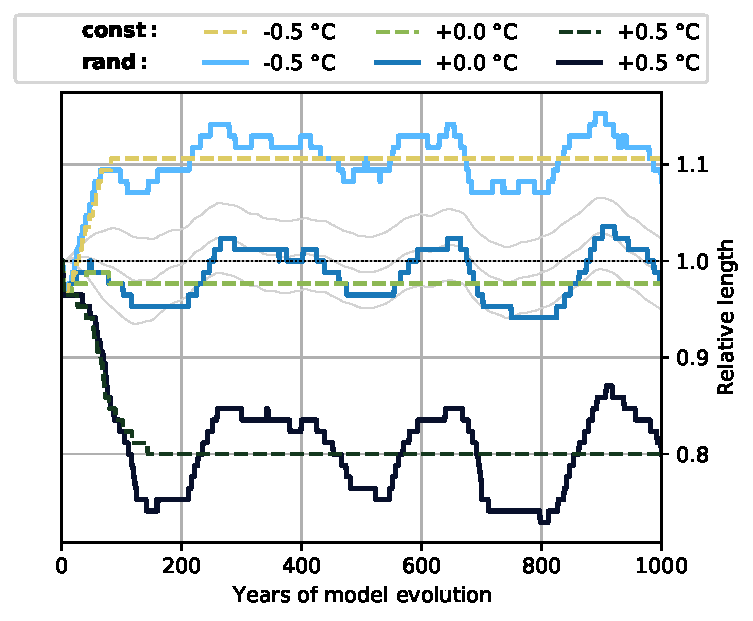
\includegraphics[width=\textwidth]{../plots/final_plots/time_series/single_glaciers/length_norm_fl_Mer_de_Glace.pdf}
  \end{subfigure}
  
  \caption{Temporal evolution of ice volume in (\subref{fig:Mer_de_Glace:volume_vas}) and (\subref{fig:Mer_de_Glace:volume_fl}), surface area in (\subref{fig:Mer_de_Glace:area_vas}) and (\subref{fig:Mer_de_Glace:area_fl}) and glacier length in (\subref{fig:Mer_de_Glace:length_vas}) and (\subref{fig:Mer_de_Glace:length_fl}) for \textbf{Mer de Glace (RGI60-11.03643)}. The shown values area normalized with their respective initial values. The left panels show the result of the \vas{} model, the right panels show the results of the flowline model. Solid lines represent the random climate scenarios, while dashed lines represent the constant climate scenarios. All climate scenarios are based on an equilibrium climate. The applied temperature biases of \SI{-.5}{\celsius}, \SI{0}{\celsius} and \SI{+.5}{\celsius} are color coded, see legend for details. The dotted line indicates the initial volume. The light gray lines represent the volume evolutions of the other model, to facilitate comparisons.}
  \label{fig:Mer_de_Glace}
\end{figure}

\begin{figure}[p]
  \centering

  % VAS volume
  \begin{subfigure}[b]{0.476\textwidth}
    \caption{\Vas{} model, relative ice volume}
    \label{fig:Glacier_d_Argentiere:volume_vas}
    \centering
    \includegraphics[width=\textwidth]{../plots/final_plots/time_series/single_glaciers/volume_norm_vas_Glacier_d'Argentière.pdf}
  \end{subfigure}
  \hfill
  % Flowline volume
  \begin{subfigure}[b]{0.476\textwidth}
    \caption{Flowline model, relative ice volume}
    \label{fig:Glacier_d_Argentiere:volume_fl}
    \centering
    \includegraphics[width=\textwidth]{../plots/final_plots/time_series/single_glaciers/volume_norm_fl_Glacier_d'Argentière.pdf}
  \end{subfigure}

  % VAS area
  \begin{subfigure}[b]{0.476\textwidth}
    \caption{\Vas{} model, relative surface area}
    \label{fig:Glacier_d_Argentiere:area_vas}
    \centering
    \includegraphics[width=\textwidth]{../plots/final_plots/time_series/single_glaciers/area_norm_vas_Glacier_d'Argentière.pdf}
  \end{subfigure}
  \hfill
  % Flowline area
  \begin{subfigure}[b]{0.476\textwidth}
    \caption{Flowline model, relative surface area}
    \label{fig:Glacier_d_Argentiere:area_fl}
    \centering
    \includegraphics[width=\textwidth]{../plots/final_plots/time_series/single_glaciers/area_norm_fl_Glacier_d'Argentière.pdf}
  \end{subfigure}

  % VAS length
  \begin{subfigure}[b]{0.476\textwidth}
    \caption{\Vas{} model, relative glacier length}
    \label{fig:Glacier_d_Argentiere:length_vas}
    \centering
    \includegraphics[width=\textwidth]{../plots/final_plots/time_series/single_glaciers/length_norm_vas_Glacier_d'Argentière.pdf}
  \end{subfigure}
  \hfill
  % Flowline length
  \begin{subfigure}[b]{0.476\textwidth}
    \caption{Flowline model, relative glacier length}
    \label{fig:Glacier_d_Argentiere:length_fl}
    \centering
    \includegraphics[width=\textwidth]{../plots/final_plots/time_series/single_glaciers/length_norm_fl_Glacier_d'Argentière.pdf}
  \end{subfigure}
  
  \caption{Temporal evolution of ice volume in (\subref{fig:Glacier_d_Argentiere:volume_vas}) and (\subref{fig:Glacier_d_Argentiere:volume_fl}), surface area in (\subref{fig:Glacier_d_Argentiere:area_vas}) and (\subref{fig:Glacier_d_Argentiere:area_fl}) and glacier length in (\subref{fig:Glacier_d_Argentiere:length_vas}) and (\subref{fig:Glacier_d_Argentiere:length_fl}) for \textbf{Glacier d'Argentière (RGI60-11.03638)}. The shown values area normalized with their respective initial values. The left panels show the result of the \vas{} model, the right panels show the results of the flowline model. Solid lines represent the random climate scenarios, while dashed lines represent the constant climate scenarios. All climate scenarios are based on an equilibrium climate. The applied temperature biases of \SI{-.5}{\celsius}, \SI{0}{\celsius} and \SI{+.5}{\celsius} are color coded, see legend for details. The dotted line indicates the initial volume. The light gray lines represent the volume evolutions of the other model, to facilitate comparisons.}
  \label{fig:Glacier_d_Argentiere}
\end{figure}

\begin{figure}[p]
  \centering

  % VAS volume
  \begin{subfigure}[b]{0.476\textwidth}
    \caption{\Vas{} model, relative ice volume}
    \label{fig:Grosser_Aletschgletscher:volume_vas}
    \centering
    \includegraphics[width=\textwidth]{../plots/final_plots/time_series/single_glaciers/volume_norm_vas_Großer_Aletschgletscher.pdf}
  \end{subfigure}
  \hfill
  % Flowline volume
  \begin{subfigure}[b]{0.476\textwidth}
    \caption{Flowline model, relative ice volume}
    \label{fig:Grosser_Aletschgletscher:volume_fl}
    \centering
    \includegraphics[width=\textwidth]{../plots/final_plots/time_series/single_glaciers/volume_norm_fl_Großer_Aletschgletscher.pdf}
  \end{subfigure}

  % VAS area
  \begin{subfigure}[b]{0.476\textwidth}
    \caption{\Vas{} model, relative surface area}
    \label{fig:Grosser_Aletschgletscher:area_vas}
    \centering
    \includegraphics[width=\textwidth]{../plots/final_plots/time_series/single_glaciers/area_norm_vas_Großer_Aletschgletscher.pdf}
  \end{subfigure}
  \hfill
  % Flowline area
  \begin{subfigure}[b]{0.476\textwidth}
    \caption{Flowline model, relative surface area}
    \label{fig:Grosser_Aletschgletscher:area_fl}
    \centering
    \includegraphics[width=\textwidth]{../plots/final_plots/time_series/single_glaciers/area_norm_fl_Großer_Aletschgletscher.pdf}
  \end{subfigure}

  % VAS length
  \begin{subfigure}[b]{0.476\textwidth}
    \caption{\Vas{} model, relative glacier length}
    \label{fig:Grosser_Aletschgletscher:length_vas}
    \centering
    \includegraphics[width=\textwidth]{../plots/final_plots/time_series/single_glaciers/length_norm_vas_Großer_Aletschgletscher.pdf}
  \end{subfigure}
  \hfill
  % Flowline length
  \begin{subfigure}[b]{0.476\textwidth}
    \caption{Flowline model, relative glacier length}
    \label{fig:Grosser_Aletschgletscher:length_fl}
    \centering
    \includegraphics[width=\textwidth]{../plots/final_plots/time_series/single_glaciers/length_norm_fl_Großer_Aletschgletscher.pdf}
  \end{subfigure}
  
  \caption{Temporal evolution of ice volume in (\subref{fig:Grosser_Aletschgletscher:volume_vas}) and (\subref{fig:Grosser_Aletschgletscher:volume_fl}), surface area in (\subref{fig:Grosser_Aletschgletscher:area_vas}) and (\subref{fig:Grosser_Aletschgletscher:area_fl}) and glacier length in (\subref{fig:Grosser_Aletschgletscher:length_vas}) and (\subref{fig:Grosser_Aletschgletscher:length_fl}) for \textbf{Großer Aletschgletscher (RGI60-11.01450)}. The shown values area normalized with their respective initial values. The left panels show the result of the \vas{} model, the right panels show the results of the flowline model. Solid lines represent the random climate scenarios, while dashed lines represent the constant climate scenarios. All climate scenarios are based on an equilibrium climate. The applied temperature biases of \SI{-.5}{\celsius}, \SI{0}{\celsius} and \SI{+.5}{\celsius} are color coded, see legend for details. The dotted line indicates the initial volume. The light gray lines represent the volume evolutions of the other model, to facilitate comparisons.}
  \label{fig:Grosser_Aletschgletscher}
\end{figure}

\begin{figure}[p]
  \centering

  % VAS volume
  \begin{subfigure}[b]{0.476\textwidth}
    \caption{\Vas{} model, relative ice volume}
    \label{fig:Rhonegletscher:volume_vas}
    \centering
    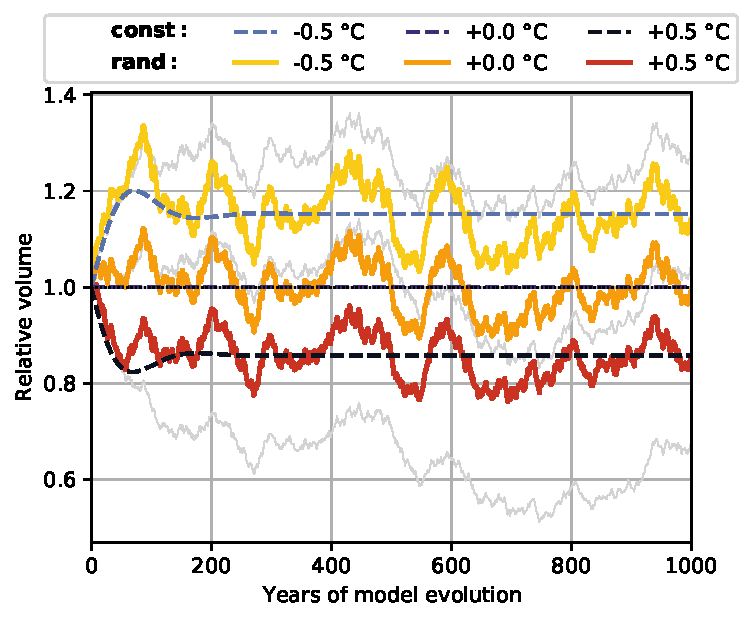
\includegraphics[width=\textwidth]{../plots/final_plots/time_series/single_glaciers/volume_norm_vas_Rhonegletscher.pdf}
  \end{subfigure}
  \hfill
  % Flowline volume
  \begin{subfigure}[b]{0.476\textwidth}
    \caption{Flowline model, relative ice volume}
    \label{fig:Rhonegletscher:volume_fl}
    \centering
    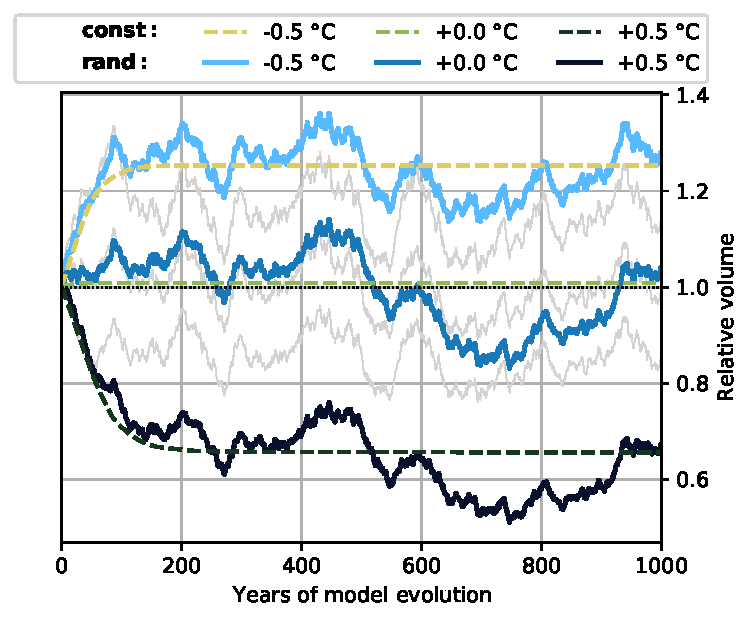
\includegraphics[width=\textwidth]{../plots/final_plots/time_series/single_glaciers/volume_norm_fl_Rhonegletscher.pdf}
  \end{subfigure}

  % VAS area
  \begin{subfigure}[b]{0.476\textwidth}
    \caption{\Vas{} model, relative surface area}
    \label{fig:Rhonegletscher:area_vas}
    \centering
    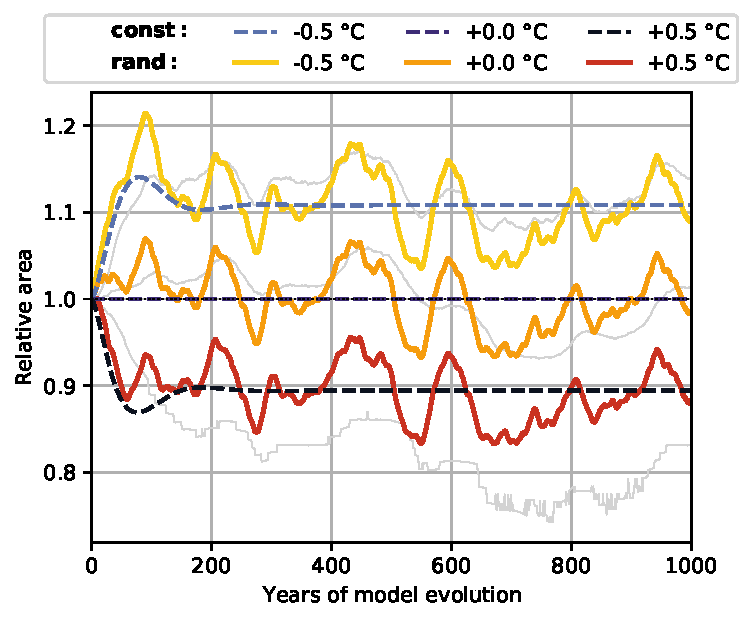
\includegraphics[width=\textwidth]{../plots/final_plots/time_series/single_glaciers/area_norm_vas_Rhonegletscher.pdf}
  \end{subfigure}
  \hfill
  % Flowline area
  \begin{subfigure}[b]{0.476\textwidth}
    \caption{Flowline model, relative surface area}
    \label{fig:Rhonegletscher:area_fl}
    \centering
    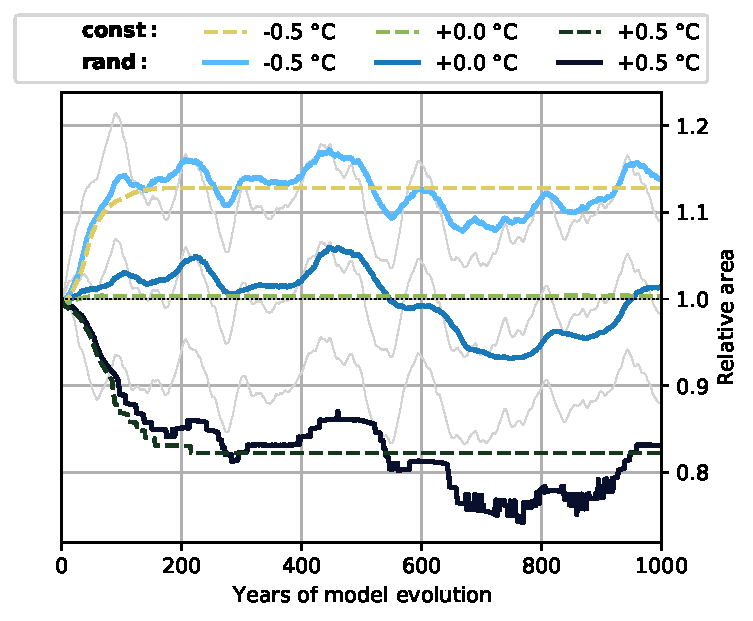
\includegraphics[width=\textwidth]{../plots/final_plots/time_series/single_glaciers/area_norm_fl_Rhonegletscher.pdf}
  \end{subfigure}

  % VAS length
  \begin{subfigure}[b]{0.476\textwidth}
    \caption{\Vas{} model, relative glacier length}
    \label{fig:Rhonegletscher:length_vas}
    \centering
    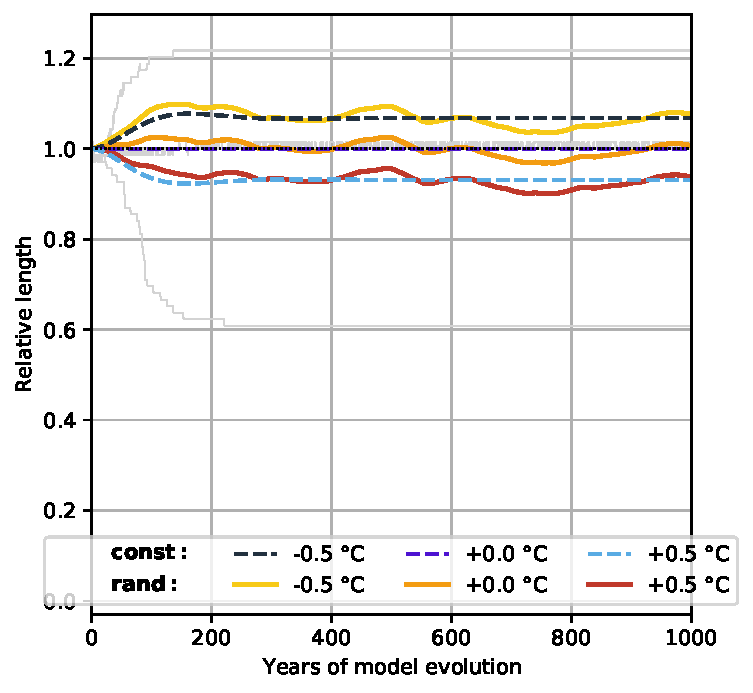
\includegraphics[width=\textwidth]{../plots/final_plots/time_series/single_glaciers/length_norm_vas_Rhonegletscher.pdf}
  \end{subfigure}
  \hfill
  % Flowline length
  \begin{subfigure}[b]{0.476\textwidth}
    \caption{Flowline model, relative glacier length}
    \label{fig:Rhonegletscher:length_fl}
    \centering
    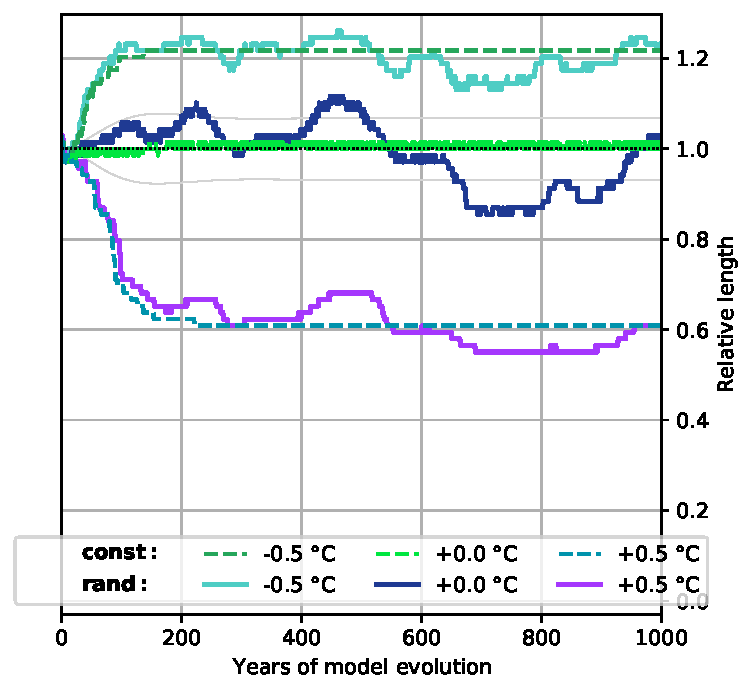
\includegraphics[width=\textwidth]{../plots/final_plots/time_series/single_glaciers/length_norm_fl_Rhonegletscher.pdf}
  \end{subfigure}
  
  \caption{Temporal evolution of ice volume in (\subref{fig:Rhonegletscher:volume_vas}) and (\subref{fig:Rhonegletscher:volume_fl}), surface area in (\subref{fig:Rhonegletscher:area_vas}) and (\subref{fig:Rhonegletscher:area_fl}) and glacier length in (\subref{fig:Rhonegletscher:length_vas}) and (\subref{fig:Rhonegletscher:length_fl}) for \textbf{Rhonegletscher (RGI60-11.01238)}. The shown values area normalized with their respective initial values. The left panels show the result of the \vas{} model, the right panels show the results of the flowline model. Solid lines represent the random climate scenarios, while dashed lines represent the constant climate scenarios. All climate scenarios are based on an equilibrium climate. The applied temperature biases of \SI{-.5}{\celsius}, \SI{0}{\celsius} and \SI{+.5}{\celsius} are color coded, see legend for details. The dotted line indicates the initial volume. The light gray lines represent the volume evolutions of the other model, to facilitate comparisons.}
  \label{fig:Rhonegletscher}
\end{figure}

\chapter{ARMA model order}\label{appendix_B}
\thispagestyle{plain}

\begin{figure}[h!]
  \centering

  % AR
  \begin{subfigure}[b]{0.5\textwidth}
    \caption{Order $p$ for the autoregressive term}
    \label{fig:arma:arp}
    \centering
    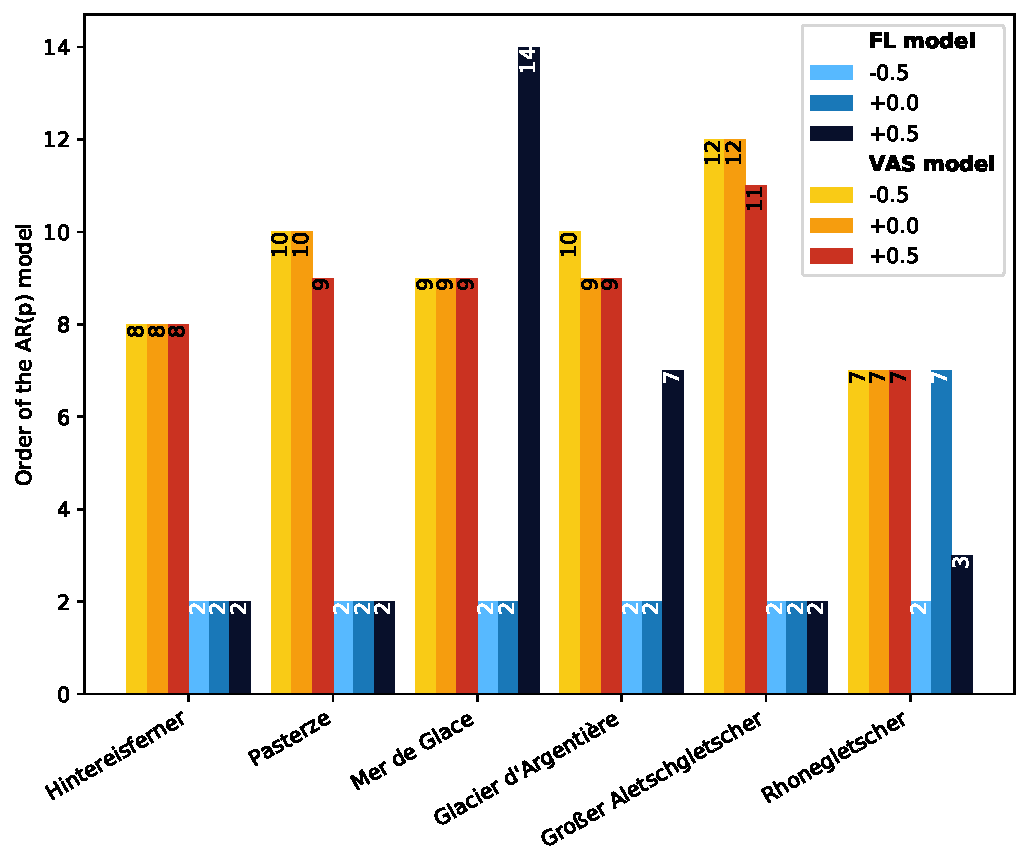
\includegraphics[width=\textwidth]{../plots/final_plots/arma/arp.pdf}
  \end{subfigure}
  \hfill
  % MA
  \begin{subfigure}[b]{0.5\textwidth}
    \caption{Order $q$ for the moving-average term}
    \label{fig:arma:maq}
    \centering
    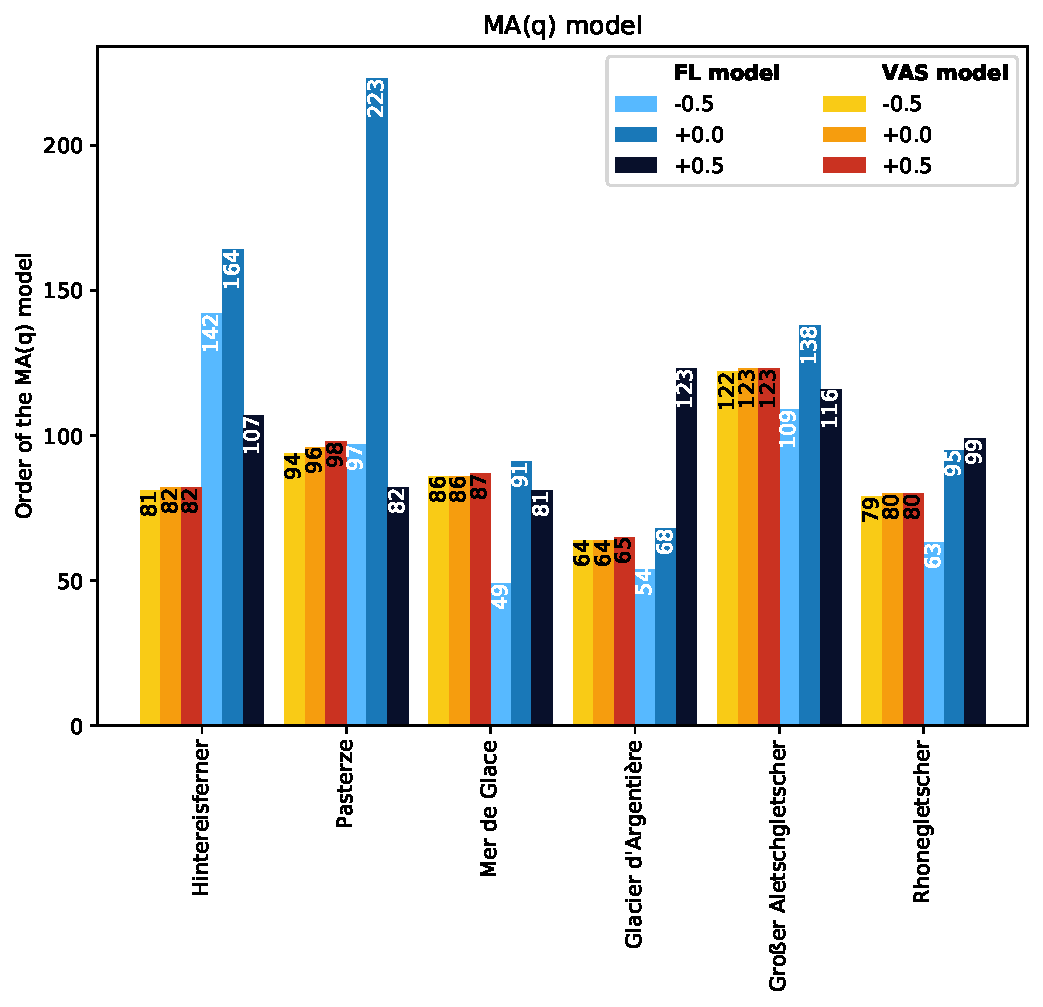
\includegraphics[width=\textwidth]{../plots/final_plots/arma/maq.pdf}
  \end{subfigure}
  
  \caption{Orders $p$ and $q$ for a potential ARMA($p$,$q$) model, estimated from the ACFs and PACFs of the length change signal in response to a white noise climate (see Section~\ref{sub:autocorrelation_function_results})}.
  \label{fig:arma}
\end{figure}


\newpage
\thispagestyle{plain}


% ==== START BACK MATTER (this has no visual effect)============================
\backmatter 


% ==== BIBLIOGRAPHY ============================================================
\addcontentsline{toc}{chapter}{Bibliography}
% ---- use AMS reference format (use file ametsoc.bst included in ...
%      ... http://www.ametsoc.org/pubs/journals/AMS_Latex_V3.0.tar.gz):s
\bibliographystyle{./ametsoc}   % ametsoc.bst in local directory
% ---- use BibTeX database file:
\bibliography{./mybibfile}      % mybibfile.bib in local directory
\newpage
\thispagestyle{plain}


% ==== ACKNOWLEDGMENTS =========================================================
% ---- include tex-file:
%!TEX root = thesis.tex
\chapter*{Acknowledgments}
\addcontentsline{toc}{chapter}{Acknowledgments}
\thispagestyle{plain}
\noindent First and foremost I want to thank my supervisor Fabien Maussion. He sparked the idea of implementing the \vas{} model during the Hacktoberfest 2018 at our institute; he gave me the liberty and the time I needed to develop and test ideas, make my own mistakes and learn from them while still providing guidance and tutelage; and most importantly, over the last couple of months he steered me towards the finish line and was an essential help in sharpening my points and in finalizing this entire project.\\[0.3cm]
\noindent Additional thanks go to Ben Marzeion for providing me with the original model code and answering some questions about the implementation and conceptual details, as well as Matthias Dusch, Jan-Hendrik Malles, Timo Rothenspieler and the entire OGGM community for helping with coding problems and providing feedback to model results.\\[0.3cm]
\noindent I would like to thank my parents and grandparents for their continued support, not only during my studies but throughout my life. Special thanks go to my fiancée Carmen for her encouragement and moral support, and also just for enduring me during the more stressful times.\\[0.3cm]
\noindent Furthermore I would like to thank everybody else not mentioned by name who contributed to this thesis in any way, shape or form: by engaging in thematic discussions about harmonic oscillations or color schemes, by calling or swinging by and providing some much needed distraction, or by motivating me when I was about to throw it all away.\\[0.3cm]
\noindent And ``last but not least'', to quote Snoop Dogg, ``I want to thank me. I want to thank me for believing in me. I want to thank me for doing all this hard work. [...] I want to thank me for never quitting.''
\newpage
\thispagestyle{plain}


% ==== CURRICULUM VITAE ========================================================
% ---- include tex-file:
%!TEX root = thesis.tex
\chapter*{Curriculum Vitae}
\addcontentsline{toc}{chapter}{Curriculum Vitae}
\thispagestyle{plain}
%
%
% ---- name, address, and date of birth:
\vspace{-0.5cm}
FirstName LastName\\
Address\\
Born on 01 April 1976 in Town, Country
\\[5mm]
%
%
% ---- education:
\textsc{Education and Professional training}:
\\[1ex]
\begin{tabular}{@{} p{2.5cm} @{} p{12.5cm} @{}}
1999--2003 &
Research assistant and Ph.D. student in the group of Dr. LastName at the
Institute of Meteorology and Geophysics, University of Innsbruck. \\[1ex]
1998--1999 &
Diploma thesis under the guidance of Dr. LastName,
Institute of Meteorology and Geophysics, University of Innsbruck:
\textit{``Title of your diploma thesis''}. \\[1ex]
1993--1998 &
Diploma study at the University of Innsbruck.
\textit{Master of Natural Science (Magister rerum naturalium)} in Meteorology.
\\[1ex]
1989--1993 &
Highschool, Town. \textit{Matura}.
\end{tabular}
\\[5mm]
%
%
% ---- training courses:
\textsc{Meteorological training courses}:
``Numerical methods and adiabatic formulation of models'', ECMWF, 1998; ``Data
assimilation and use of satellite data'', ECMWF, 1998.
\\[5mm]
%
%
% ---- field experiments:
\textsc{Participation in field experiments}:
Gap flow study (MAP), Austria, 1999.

\newpage
\thispagestyle{plain}


% ==== EPILOGUE ================================================================
% ---- include tex-file:
%!TEX root = thesis.tex
\chapter*{Epilogue}
\addcontentsline{toc}{chapter}{Epilogue}
\thispagestyle{plain}

Here is the place where you may want to tell a little story or a fairy tale
which has some relevance for your thesis, such as ``Once upon a time, \dots''.
The Epilogue is optional.

\newpage
\thispagestyle{plain}


\end{document}
% ==== END OF BODY =============================================================
